%Type of Document
\documentclass[a4paper, 12pt]{report}

%Load Pre-ambles
\usepackage{../Environment/Packages}
\usepackage{../Environment/Conventions}
\usepackage{../Environment/Hyahoos}
\def\sizes{0.15}

\begin{document}

\begin{center}
%Seperator
%Seperator
%Seperator
\section{Problem 4}
\begin{comment}
\end{comment}
Reiterating Euler's equations of motion,
$$\begin{bmatrix}M_x \\ M_y \\ M_z\end{bmatrix} = \begin{bmatrix} 
I_{x}\dot{\w_x} + (I_{z} - I_{y})\w_z\w_y\\
I_{y}\dot{\w_y} + (I_{x} - I_{z})\w_x\w_z\\
I_{z}\dot{\w_z} + (I_{y} - I_{x})\w_x\w_y
\end{bmatrix}$$
%Seperator
%Seperator
\subsection{Part a}
Assuming no torque-free motion,
$$M_x = 0 \quad,\quad M_y = 0 \quad,\quad M_z = 0$$
Assuming the symmetry conditions, $I_x = I_y = I_t$,
$$I_{y} - I_{x} = 0$$
In the $z$-direction,
$$0 = I_{z}\dot{\w_z}$$
Since $I_z\neq 0$, then
$$0 = \dot{\w_z}$$
This means that $\w_z$ is a constant in time, let $\w_z = \Omega$, at time $t=0$. Then it must follow,
$$\w_z = \Omega$$
for all time $t$. Let $I_z = I_a$. Substituting these assumptions and findings into the $x$ and $y$ direction of Euler's equations of motion,
$$0 = I_{t}\dot{\w_x} + (I_{a} - I_{t})\Omega\w_y \quad,\quad 0 = I_{t}\dot{\w_y} + (I_{t} - I_{a})\w_x\Omega$$
Re-arranging the equations,
$$0 = \dot{\w_x} + \f{(I_{a} - I_{t})}{I_{t}}\Omega\w_y \quad,\quad 0 = \dot{\w_y} + \f{(I_{t} - I_{a})}{I_{t}}\w_x\Omega$$
Differentiating both equations with respect to time,
$$0 = \ddot{\w_x} + \f{(I_{a} - I_{t})}{I_{t}}\Omega\dot{\w_y} \quad,\quad 0 = \ddot{\w_y} + \f{(I_{t} - I_{a})}{I_{t}}\dot{\w_x}\Omega$$

Substituting the second order derivative $\w_x$ into the first order derivative $\w_y$,
$$\dot{\w_y} = -\f{(I_{t} - I_{a})}{I_{t}}\w_x\Omega$$
$$0 = \ddot{\w_x} + \f{(I_{a} - I_{t})}{I_{t}}\Omega\dot{\w_y} = \ddot{\w_x} - \f{(I_{a} - I_{t})\Omega}{I_{t}}\f{(I_{t} - I_{a})\Omega}{I_{t}}\w_x = \ddot{\w_x} + \f{(I_{t}-I_{a})^2\Omega^2}{I_{t}^2}\w_x = \ddot{\w_x} + \l[\f{(I_{t}-I_{a})\Omega}{I_{t}}\r]^2\w_x$$

Therefore, the characteristic equation to the differential equation above,
$$0 = r^2 + \l[\f{(I_{t}-I_{a})\Omega}{I_{t}}\r]^2$$
$$r^2 =  - \l[\f{(I_{t}-I_{a})\Omega}{I_{t}}\r]^2$$
$$r =  \pm \l[\f{(I_{t}-I_{a})\Omega}{I_{t}}\r]i$$
Let $\dst{\la = \f{(I_{t}-I_{a})\Omega}{I_{t}}}$, then $r = \pm\la i$. By some choice of arbitrary constants, the solution to the differential equation,
$$\w_x = A\cos(\la t) + B\sin(\la t)$$
When $t=0$, $\w_x$ = $\w_{x,o}$
$$\w_{x,o} = A$$
Taking the derivative of $\w_x$,
$$\dot{\w_x} = A\f{d}{dt}[\cos(\la t)] + B\f{d}{dt}[\sin(\la t)] = A\times-\sin(\la t)\times \la + B\cos(\la t)\times \la = -A\la\sin(\la t)  + B\la\cos(\la t)$$
When $t=0$, $\dot{\w_x} = \dot{w_{x,o}}$. Substituting,
$$\dot{\w_{x,o}} = B\la$$
$$B = \f{\dot{\w_{x,o}}}{\la}$$

Substituting for $A$ and $B$ to form the solution $\w_x$,
$$\w_x = A\cos(\la t) + B\sin(\la t) = \w_{x,o}\cos(\la t) + \f{\dot{\w_{x,o}}}{\la}\sin(\la t)$$

Re-writing Euler's equations of motion in terms of $\la$ for $\w_y$,
$$0 = \dot{\w_x} + \f{(I_{a} - I_{t})}{I_{t}}\Omega\w_y$$
$$\dot{\w_x} =  - \f{(I_{a} - I_{t})}{I_{t}}\Omega\w_y = \f{(I_{t} - I_{a})\Omega}{I_{t}}\w_y = \la\w_y$$
$$\w_y = \f{\dot{\w_x}}{\la} = \f{1}{\la}\f{d}{dt}\l[\w_{x,o}\cos(\la t) + \f{\dot{\w_{x,o}}}{\la}\sin(\la t)\r] = \f{1}{\la}\l[-\w_{x,o}\la\sin(\la t) + \dot{\w_{x,o}}\cos(\la t)\r]$$
$$\w_y = -\w_{x,o}\sin(\la t) + \f{\dot{\w_{x,o}}}{\la}\cos(\la t)$$

Since $\dst{\dot{\w_x} = \la\w_y}$, $\dst{\dot{\w_{x,o}} = \la\w_{y,o}}$. Manpulating, $\dst{\f{\dot{\w_{x,o}}}{\la} = \w_{y,o}}$. Substituting, into the rotation $\w_x$,
$$\w_x = \w_{x,o}\cos(\la t) + \w_{y,o}\sin(\la t)$$
Substituting into the rotation $\w_y$,
$$\w_y = -\w_{x,o}\sin(\la t) + \w_{y,o}\cos(\la t)$$

Here the results differ slightly due to the slightly different formulation of $\la$. To reconcile the results to the lecture results, let $\la_l = -\la$, wherein $\la_l$ is the $\la$ defined in the lecture, substituting,
$$\w_x = \w_{x,o}\cos(-\la_l t) + \w_{y,o}\sin(-\la_l t) \quad,\quad \w_y = -\w_{x,o}\sin(-\la_l t) + \w_{y,o}\cos(-\la_l t)$$
\\~\\\fbox{$\dst{\w_x = \w_{x,o}\cos(\la_l t) - \w_{y,o}\sin(\la_l t) \quad,\quad \w_y = \w_{x,o}\sin(\la_l t) + \w_{y,o}\cos(\la_l t)}$}


%Seperator
%Seperator
\subsection{Part b}
The diagram of the ${}^{e}\w^{b}$ as well as the body cone is shown below,
\\~\\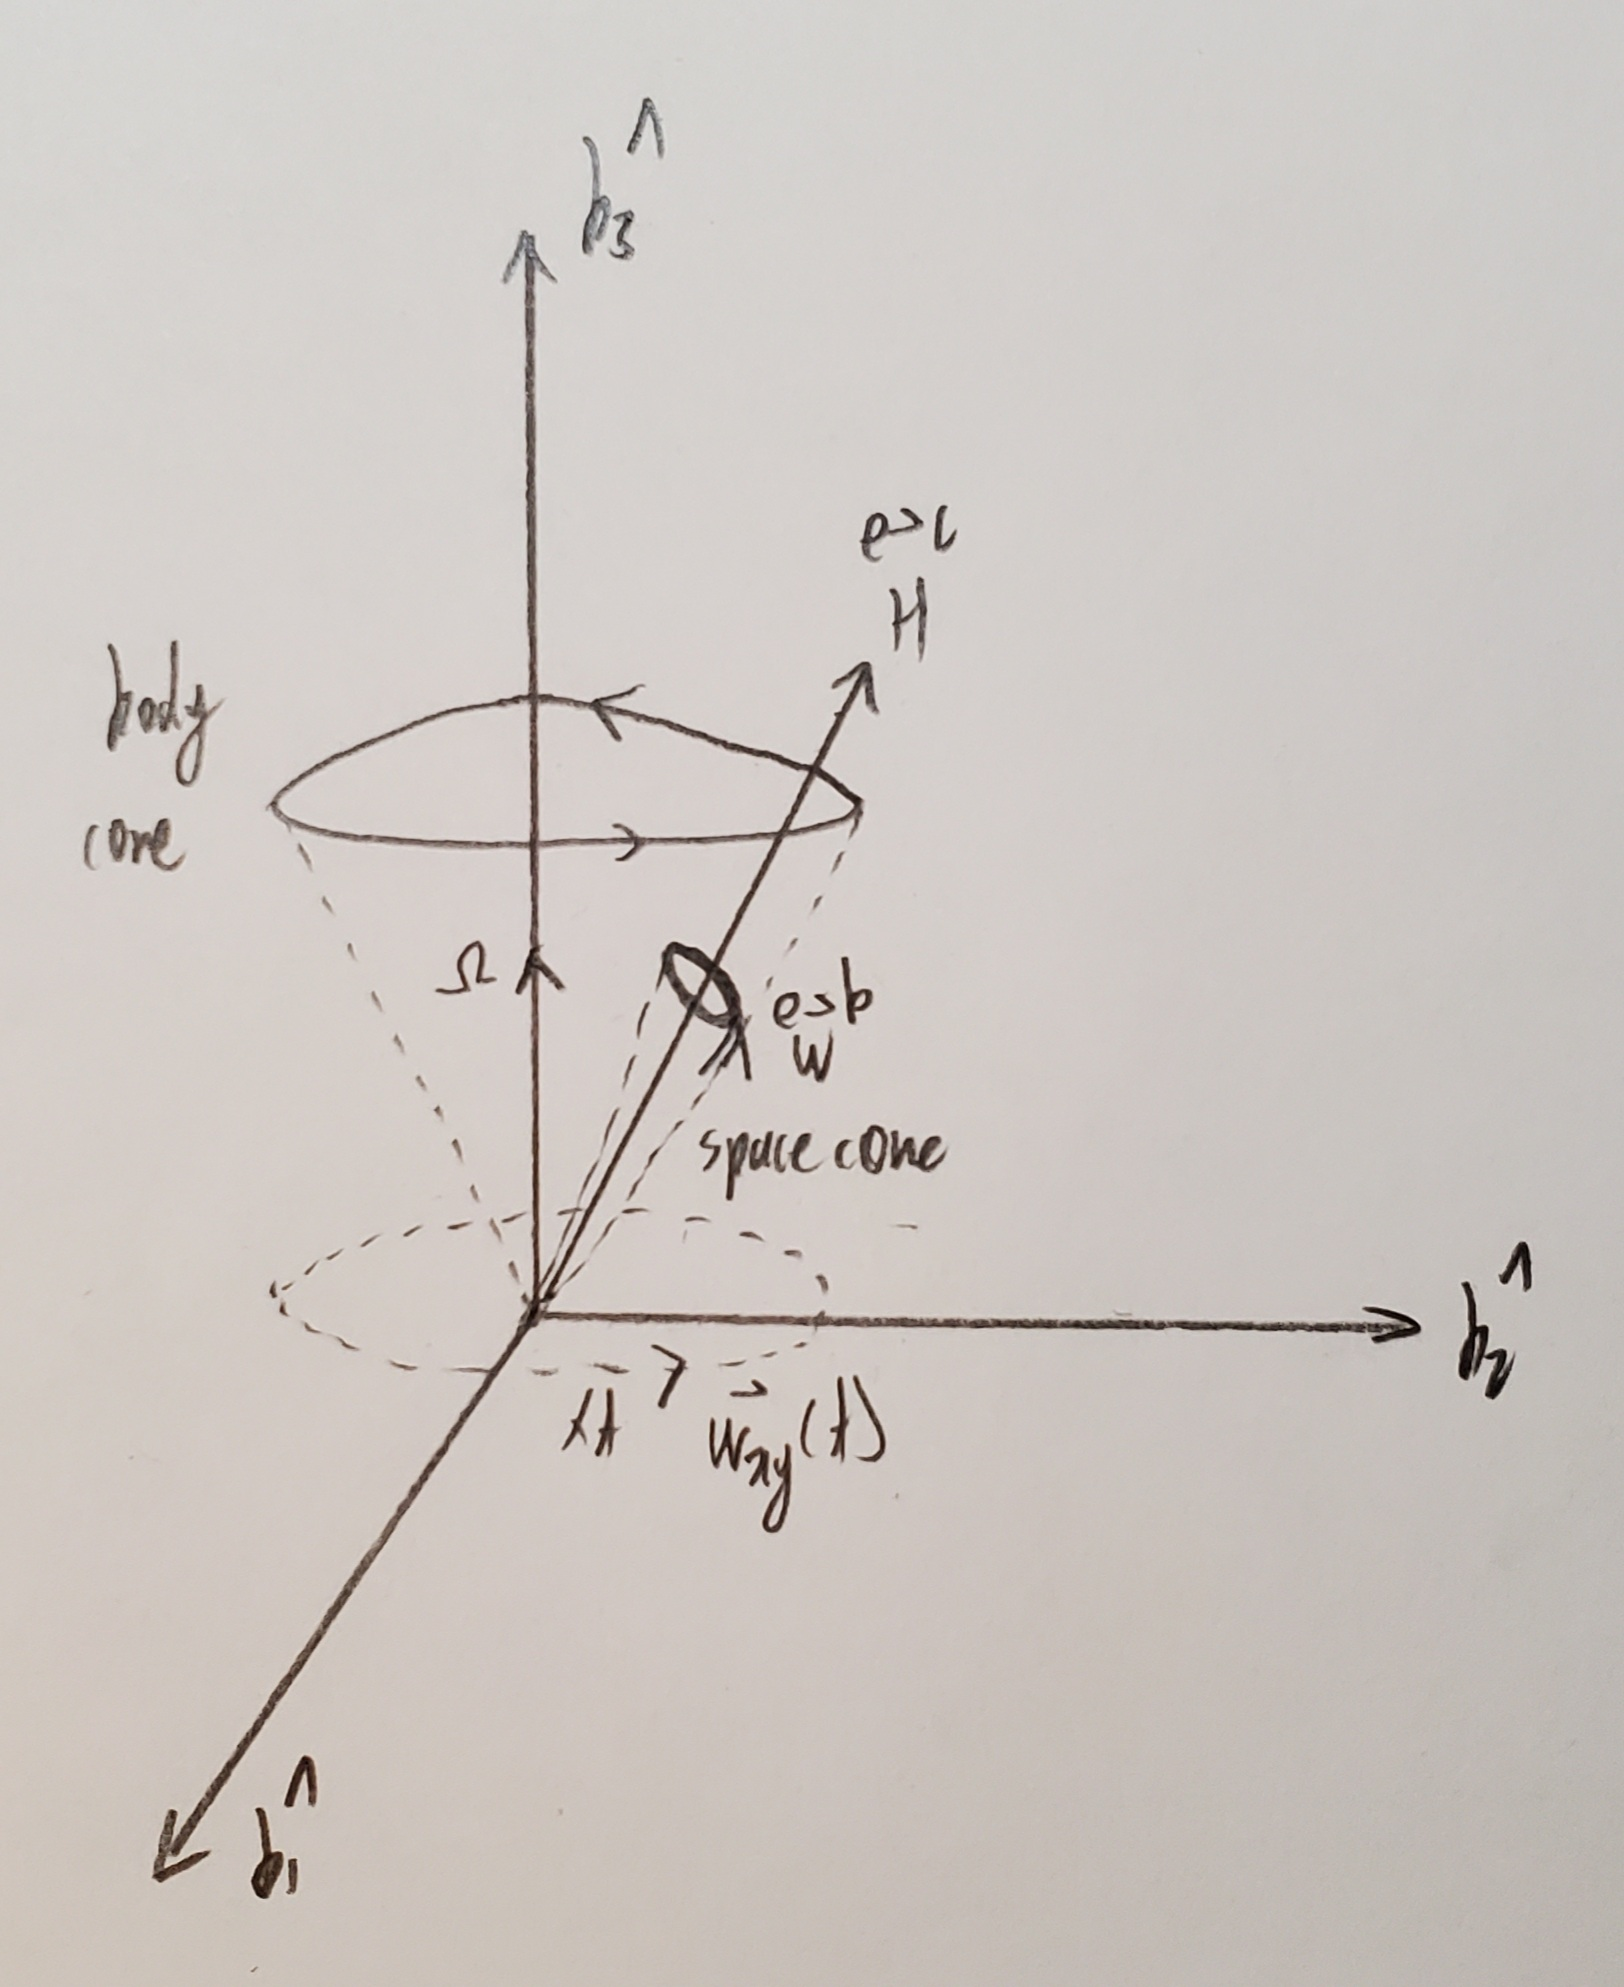
\includegraphics[scale=\sizes]{Bajingan}
%Seperator
%Seperator
\subsection{Part c}
The angular velocity vector,
$$\b{\w} = \begin{bmatrix}\w_x && \w_y && \w_z\end{bmatrix}^T$$
Substituting, for the results from the previous part a,
$$\b{\w} = \begin{bmatrix}
\w_{x,o}\cos(\la_l t) - \w_{y,o}\sin(\la_l t) \\
\w_{x,o}\sin(\la_l t) + \w_{y,o}\cos(\la_l t) \\
\Omega
\end{bmatrix}$$
This could be re-arranged into the following matrix equation,
$$\b{\w} = A\b{I_c} =\begin{bmatrix}
\cos(\la_l t) && -\sin(\la_l t) && 0\\
\sin(\la_l t) && \cos(\la_l t) && 0\\
0 && 0 && 1
\end{bmatrix}\begin{bmatrix}
\w_{x,o} \\ \w_{y,o} \\ \Omega
\end{bmatrix}$$
\\~\\\fbox{\parbox{\textwidth}{
wherein the matrix $A$ represents the rotation matrix about axis $z$ and $\b{I_c}$ represent the initial conditions of the problem. Typically the rotation matrix accepts arguments $\t$ wherein $\t$ represents the angle of rotation in the counter-clockwise direction. As shown above, the arguments of the trigonometric function is instead $\la_l t$. As long as $\la_l>0$, then the angular velocity vector would rotate counter-clockwise. If $\la_l<0$, then the angular velocity vector would rotate in the clockwise direction.
\\~\\By re-formulating the angular velocity vector as a rotation matrix, it is proven that the angular velocity vector rotates about the $z$-axis of the body frame in the counter clockwise direction at a rate $\la_l$}}
%Seperator
%Seperator
%Seperator




\end{center}

\end{document}
